\documentclass[a4paper, 12pt]{article}

\usepackage[margin=2.5cm]{geometry}
\usepackage{indentfirst}
\usepackage{graphicx}
\usepackage{wrapfig}
\usepackage{amsmath}
\usepackage{mathrsfs}
\usepackage{icomma}

\newcommand{\parbreak}{\vspace{1cm}}

\newcommand{\figcaption}[2]{\scriptsize{\textbf{Fig. #1} #2}}

\newcommand{\lorentzradical}{\sqrt{1 - \frac{V^2}{c^2}}}

\begin{document}

\section{Cinematica relativistă. Consecințele cinematice \\ ale transformărilor Lorentz}

\subsection{Contracția relativistă a lungimilor}
\par
În mecanica clasică, conform transformărilor Galilei, se aplică invarianța
intervalului spațial, adică dimensiunile corpurilor rămân constante la
trecerea de la un SRI la altul.

Intervalul temporal este de asemenea considerat invariant la trecerea
de la un SRI la altul.

Însă timpul și spațiul nu mai pot fi considerate mărimi absolute în teoria
relativității creată de Einstein.

Prin trecerea de la un SRI la altul, dimensiunile longitudinale ale corpurilor
suferă modificări.

\parbreak

De exemplu, considerăm un corp de formă liniară, precum o riglă, aflată pe axa
$Ox$ în repaus și având lungimea $l_0$ în sistemul S, numit
\emph{sistem de referință propriu} (SRP). Putem exprima $l_0$ prin diferența
absciselor capetelor sale:
\[ l_0 = x_2(t) - x_1(t) \]

\newcommand{\betalorentzradical}{\sqrt{1 - \beta^2}}

Mai departe, măsurăm lungimea riglei în sistemul de referință inerțial $S'$,
care are o mișcare de translație uniformă de-a lungul $Ox$ cu viteza $V$ față de $S$.
Fie $x_1'$ și $x_2'$ abscisele riglei măsurate la același moment de timp $t'$,
măsurat cu un ceas solidar cu $S'$. Conform transformărilor Lorentz, obținem
\[
    l_0 = x_2 - x_1
    = \frac{x_2' + Vt'}{\betalorentzradical} - \frac{x_1' + Vt'}{\betalorentzradical}
    = \frac{x_2' - x_1'}{\betalorentzradical} = \frac{l'}{\betalorentzradical},
\]
unde am notat \( \beta = \frac{V}{c} \). De aici rezultă
\[ l' = l_0 \betalorentzradical \]

Se observă că lungimea $l'$ măsurată în $S'$ este mai mică decât lungimea
proprie $l_0$. Rigla a rămas identică cu ea însăși, însă rezultatul măsurării
lungimii diferă de la un SRI la altul.

\pagebreak

{\Large\emph{Problemă rezolvată}}
\vspace{0.5cm}

Fie o riglă aflată în repaus într-un SRI $S'$, care este aflat în translație
uniformă față de un SRI $S$. Să se exprime lungimea riglei \( l = x_2(t) - x_1(t) \)
în referențialul $S$ în funcție de lungimea \( l' = l_0 \)
a riglei în sistemul $S'$.

\begin{figure}[h]
    \centering
    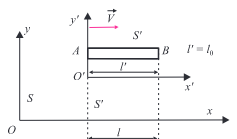
\includegraphics[width=0.5\textwidth]{fig/rigla} \\
    \figcaption{1}{Contractarea lungimilor. Rigla este solidară cu $S'$}
\end{figure}

Din \( x' = \dfrac{x - Vt}{\lorentzradical} \)
rezultă \( x = x' \lorentzradical + Vt \). Atunci:
\begin{align*}
    l &= x_2' \lorentzradical + Vt - x_1' \lorentzradical - Vt \\
    l &= (x_2' - x_1') \lorentzradical = l_0 \lorentzradical < l_0
\end{align*}

\parbreak

Dimensiunile transversale ale corpurilor nu se modifică: \( y' = y \) și \( z' = z \).
Astfel, volumul corpului se modifică doar în direcția mișcării:
\[ \mathscr{V}_0 = xyz \]
\[ \mathscr{V}' = x'y'z' = x\lorentzradical yz = \mathscr{V}_0 \lorentzradical \]

\begin{wrapfigure}{r}{0.4\textwidth}
    \centering
    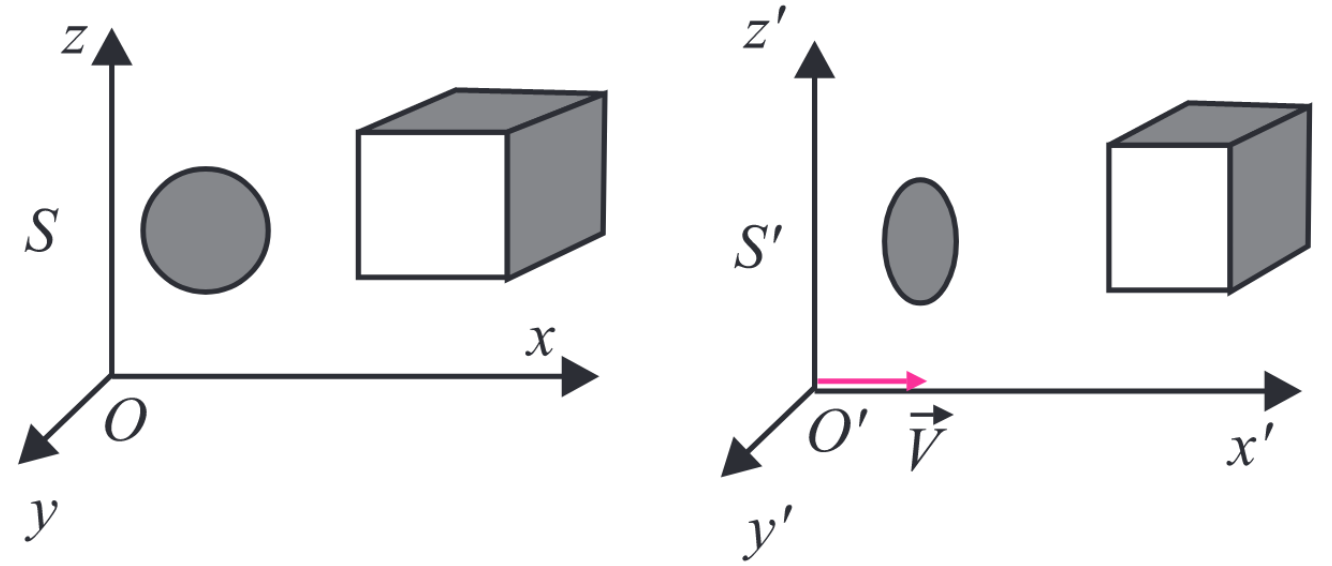
\includegraphics[width=0.5\textwidth]{fig/turtit.png}
    \figcaption{2}{Sfera se turtește, iar cubul se transformă în paralelipiped}
\end{wrapfigure}

Privind o sferă dintr-un sistem de referință față de care se mișcă, aceasta
apare turtită în direcția mișcării. Un cub devine un paralelipiped.
Aceste modificări reprezintă forma reală a obiectelor, nu doar ceea ce vede
un observator. Imaginea adevărată a corpului poate fi obținută numai prin
localizarea simultană a tuturor punctelor acestuia. Atunci când observăm un
obiect în mișcare rapidă, în realitate înregistrăm fotonii emiși de obiect
atunci când ajung pe retină. Fotonii nu au fost emiși simultan de toate punctele
corpului, și astfel ochiul percepe o imagine deformată.

Dacă viteza corpului ar fi \( V = c \), dimensiunea sa longitudinală s-ar reduce
la zero, corpul degenerând într-un plan transversal față de $Ox$.

Prin urmare, concepția spațiului absolut \( \left( l' = l_0 \right) \) este
înlocuită în teoria relativistă de concepția spațiului relativ, reprezentată
de relația \( l' = l_0 \lorentzradical \). Orice dimensiune poate fi cunoscută
numai în mărime relativă.

Pentru \( V \rightarrow 0 \), avem \( \lorentzradical \rightarrow 1 \) și deci
relația clasică \( l' = l_0 \).

Pentru \( V > c \), radicalul lui Lorentz devine imaginar, iar noțiunea de lungime
își pierde sensul.

\subsection{Dilatarea relativistă a timpului}
Pe semiaxa $Ox$ a sistemului $S$, considerăm un eveniment temporar cu durata
\[ \tau_0 = t_2(x) - t_1(x) \]

$\tau_0$ mai este numit și timp propriu.

Durata acestui eveniment, măsurată în sistemul $S'$ aflat în mișcare față de
$S$, este egală cu diferența momentelor respective în $S'$ luate pentru aceeași
abscisă $x$:
\[ \tau' = t_2'(x) - t_1'(x) \]

Din \( t' = \dfrac{t - \frac{Vx}{c^2}}{\lorentzradical} \) rezultă:
\[
    \tau'
    = \frac{t_2 - \frac{Vx}{c^2}}{\lorentzradical}
    - \frac{t_1 - \frac{Vx}{c^2}}{\lorentzradical}
    = \frac{t_2 - t_1}{\lorentzradical} = \frac{\tau_0}{\lorentzradical} > \tau_0
\]

Prin urmare, durata $\tau'$ măsurată în sistemul $S'$ a unui eveniment într-un
punct aflat în mișcare față de $S'$ este mai mare decât durata $\tau_0$
măsurată în sistemul $S$, față de care punctul se află în repaus:
\( \tau' > \tau_0 \).

De aici rezultă că durata unui eveniment este minimă măsurată față de sistemul
de referință propriu.

\parbreak

Dependența intervalului de timp de sistemul de referință nu este intuitivă în
comparație cu fenomenele pe care le observăm zi de zi în regim nerelativist,
când \( V \ll c \).  Un exemplu îl reprezintă prezența miuonilor la nivelul
solului sau mării. Miuonii, care apar în atmosferă la altitudini de 10 km,
datorită razelor cosmice ce pătrund în atmosfera planetei, au un timp de viață
propriu -- cel măsurat în SRP -- extrem de scurt, \( \tau_0 = 2,2 \cdot 10^{-6} \)
s. Având viteza \( V = 2,994 \cdot 10^8 \) m/s (valoare apropiată de viteza
luminii), din calculul nerelativist al distanței rezultă că un miuon ar putea
parcurge doar \( V\tau_0 = 658,7 \) m în intervalul de timp propriu, distanță
insuficientă pentru a ajunge la nivelul solului.  Deoarece observația se face
în raport cu Pământul, trebuie să luăm în considerație intervalul de timp
măsurat față de Pământ:

\[
    \tau = \frac{\tau_0}{\lorentzradical}
    = \frac{2,2 \cdot 10^{-6}}{\sqrt{1 - \left( \frac{2,994}{2,9979} \right)^2}}
    = 43,14 \cdot 10^{-6} ~ \mathrm{s}
\]

Calculând acum distanța parcursă de miuon față de Pământ, obținem:
\[ D = c\tau = 12,933 ~ \mathrm{km} \]

Rezultă că miuonul poate fi reperat la nivelul solului și chiar al mării.

\pagebreak

Pentru \( V \ll c \) se obține \( \tau = \tau_0 \), ca în mecanica clasică.

Pentru \( V \rightarrow c \), dimensiunile longitudinale ale corpurilor tind
către 0, iar intervalul de timp către infinit.

Pentru \( V = c \), corpul este redus la un plan transversal pe direcția
mișcării, iar intervalul de timp devine infinit.

Pentru \( V > c \), transformările Lorentz devin imaginare și își pierd
sensul fizic, demonstrând că viteza luminii în vid nu poate fi atinsă de
corpuri.

În concluzie, pentru un observator aflat în mișcare față de locul unde se
produce un fenomen, acesta se desfășoară mai lent decât pentru un observator
aflat în repaus față de eveniment.

\end{document}
